% Chapter Template

\chapter{Background} % Main chapter title

\label{chp:background} % Change X to a consecutive number; for referencing this chapter elsewhere, use~\ref{ChapterX}

This chapter includes required background to understand the thesis proposal presented in the following chapters.

\section{Convolutional Neural Networks (CNN)}

CNN is initially introduced by LeCun \cite{lecun1989handwritten} which is based on learning adaptive convolutional kernels. CNN consist of two parts convbase and densebase parts. For the Convbase instead of connecting all of the units in a layer to all the units in a preceding layer, convolutional networks organize each layer into feature maps \cite{lecun1989handwritten}, which
can be though of as parallel planes or channels. In a convolutional layer, the weighted sums are only performed within a small local window \textit{i.e)} receptive field, and weights are identical for all pixels, just as in regular shift-invariant image convolution and correlation. This parameter sharing reduce the required total number of parameter and allows learning shift invariant convolutional kernels. These convolutional kernels produce equivariant features maps. Fig.~\ref{lenet} represents typical CNN architecture of LeNet.
\begin{figure}
    \begin{center}
        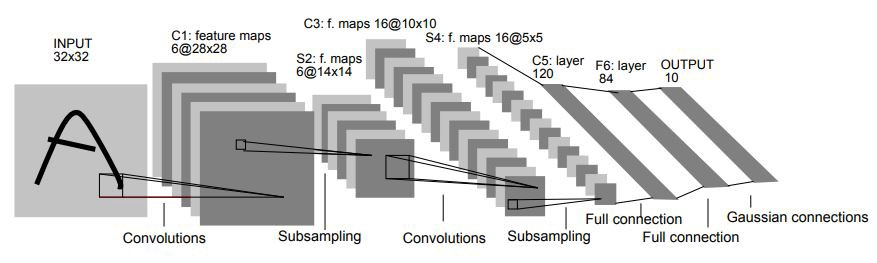
\includegraphics[width=\textwidth]{Figures/LeNetCNN.jpeg}
        \caption{Typical CNN architecture}
        \label{lenet}
    \end{center}
\end{figure}
\subsection{Convolutional Layer}
The building block of the convolutional layer is the 2D convolutional kernel. Fig.~\ref{conv2Dlayer} illustrates the 2D convolutional layer. Each 2D convolution kernel takes as input all of the $C_{i-1}$ channels in the preceding layer, windowed to a small area, and produces the values in one of the $C_{i}$ channels in the next layer. For each of the output channels, we have $K^2\times C_{i-1}$ kernel weights, so the total number of learnable parameters in each convolutional layer is $K^2\times C_{i-1} \times C_{i}$. In Fig.~\ref{conv2Dlayer}, we have $C_{i-1} = 6$ input channels and $C_{i} = 4$ output channels, with an $K = 3$ convolution window, for a total of $9 \times 6 \times 4$ learnable weights, shown in the middle column of the figure. Since the convolution is applied at each of the $W \times H$ pixels in a given layer, the amount of computation (multiply-adds) in each forward and backward pass
over one sample in a given layer is $W\times H \times K^{2} \times C_{i-1} \times C_{i}$.
To fully determine the behavior of a convolutional layer, we still need to specify the following hyperparameter:
\begin{itemize}
    \item \textbf{Padding.} Padding is used to preserve the spatial dimension of the input feature map after the convolution operation is performed. Typically, it is performed by inserting $\lfloor K/2 \rfloor$ columns for both sides and $\lfloor K/2 \rfloor$ rows to the top and bottom.
    \item \textbf{Stride.} Stride is the step taken between two centers when performing the convolution operation. Typically, Stride is equal to $1$. Stride can act as down sampling operation that can be performed instead of the pooling operation.
    \item \textbf{Dilation.} Dilation is a technique that enlarge the kernel by inserting zeros between its consecutive elements. As a result it covers a larger area of the input without increasing the total number of parameters. Which can be discribed as \[y[i]=\sum_{k}^{K} x[i+r\times k] w[k]\] where $x$ is the input signal, $w$ is the convolutional filter with size of $K$, $y$ is the resultant signal, and $r$ is the dilation rate.
\end{itemize}

\begin{figure}
    \begin{center}
        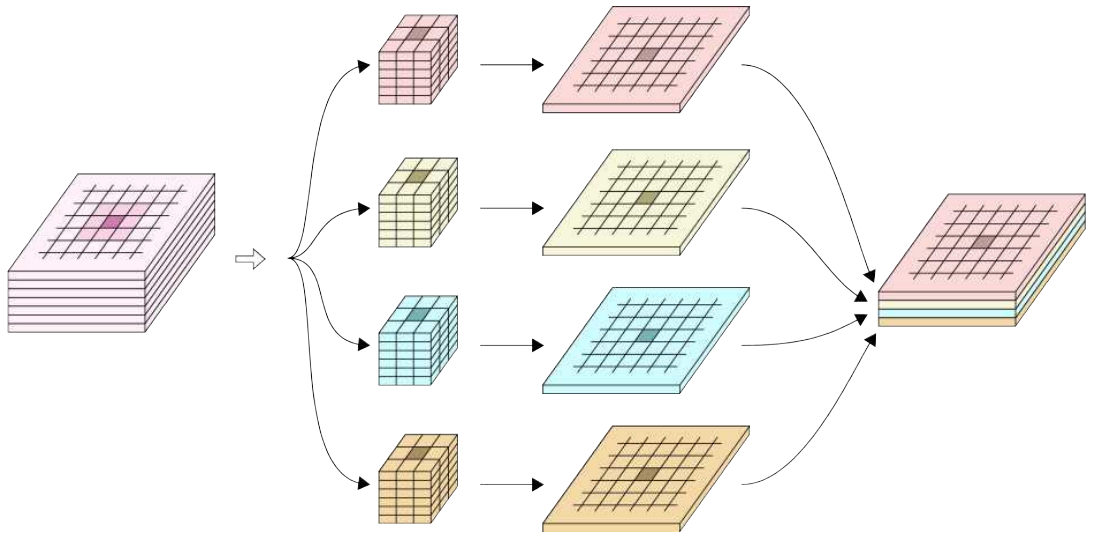
\includegraphics[width=\textwidth]{Figures/2DConvKernels.png}
        \caption{Convolutional layer with single input feature map and four convolutional kernels}
        \label{conv2Dlayer}
    \end{center}
\end{figure}


Generally, each convolutional layer computes some activation based on its input and a nonlinear function. Activation function used in each layer have a great effect on the modeling of the problem and also the semantic assigned to the output of some units is affected by this choice. The most important activation functions will be introduced in the following section.

\section{Activation functions}\label{sec:activations}
\begin{figure}
\centering
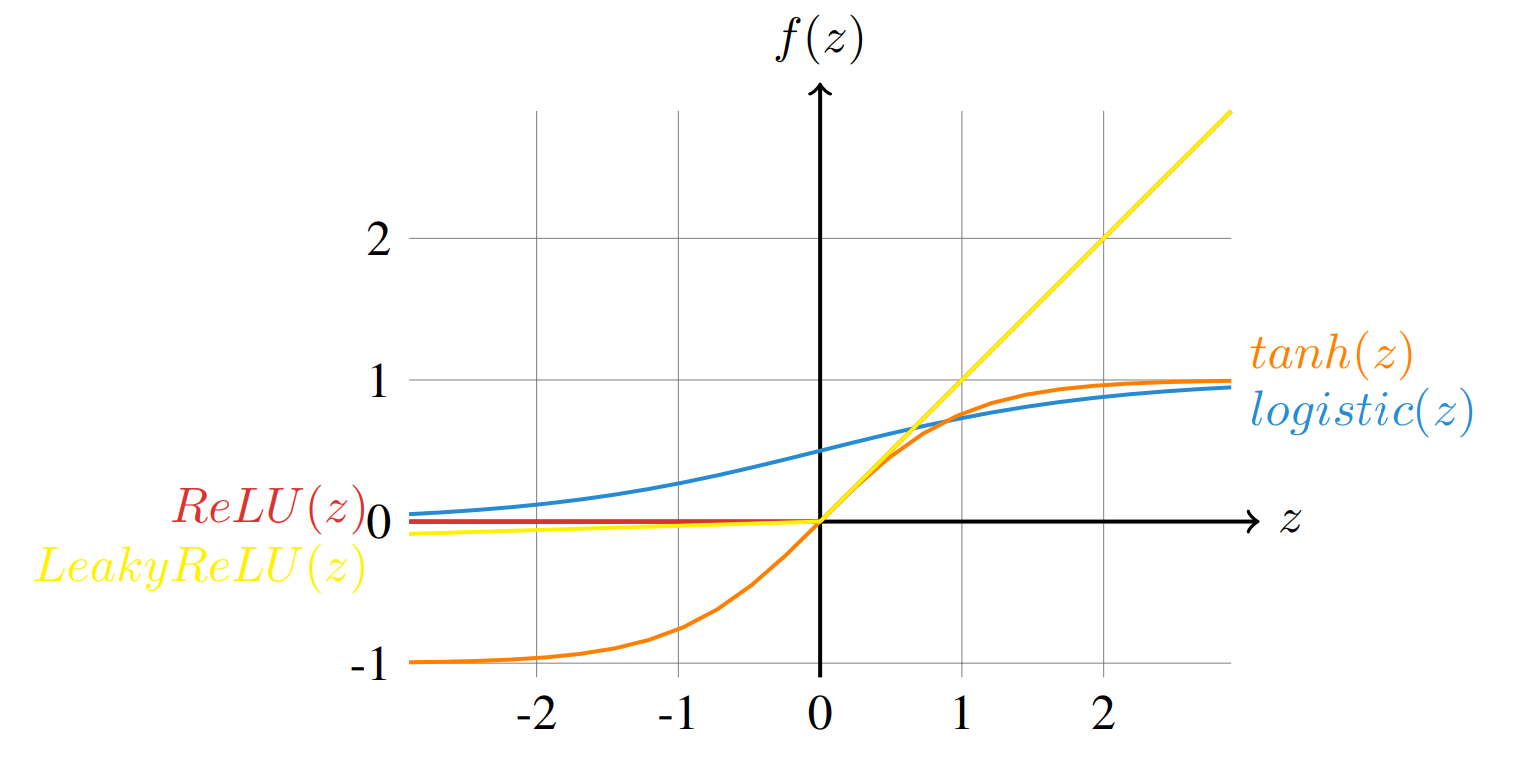
\includegraphics[width=\textwidth]{Figures/Actfuncs.png}
\caption{Some of the most common activation functions: sigmoid, tanh, ReLU and Leaky ReLU. ReLU and Leaky ReLU are overlapping for $z \geq 0$.}
\label{fig:activations}
\end{figure}

The activation function is one of the most important component of an CNN. To tackle non-linearly separable problems it is imperative to map the input into a space that is linearly separable. The activation function does this by performing an \emph{element-wise nonlinear transformation} of the pre-activation that comes from the linear combination of the convolutional layer.

The linear combination of the convolutional layer and the nonlinearity work together closely: the latter is usually fixed and does not evolve during training, but maps its input to a highly non-linear space; the former, is determined by the learned weights which is learned during the training process and uses the activation function to map the calculated activation into a new space where they are simpler and easier to separate. It is interesting to point out that $N$ consecutive linear combination is a single linear combination. Activation function breaks this property and low introducing deeper networks.

In the following subsection common activation function is presented.

\subsection{Sigmoid}\label{sec:logistic}
The sigmoid, often called \emph{logistic}, is a differentiable monotonically
increasing function that takes any real-valued number and maps it to $[0, 1]$.
As illustrates in its representation in Fig.~\ref{fig:activations}, for large
negative numbers it approaches $0$. However, for large positive numbers it
approaches to $1$. It is defined as

\begin{equation}\label{eq:logistic}
    logistic(\mathbf{z}) = \frac{1}{1+\exp(-\mathbf{z})}.
\end{equation}

\noindent The logistic function is the most used nonlinearity historically due to its possible interpretation as the firing probability of a neuron given its activation: when the activation is low the neuron fires less often whereas when the activation is high the frequency of the spikes increases.

Another very important property of the logistic function is that it is a very
simple and fast derivative computation such as follows:

\begin{align}\label{eq:logistic_derivative}
\begin{split}% to show one label only
    \frac{\partial}{\partial \mathbf{z}}logistic(\mathbf{z}) &=
        \frac{\exp(\mathbf{-z})}{\left(1+\exp(-\mathbf{z})\right)^2} ,\\
    &= \frac{1}{1+\exp(-\mathbf{z})} \cdot
        \frac{\exp(-\mathbf{z})}{1+\exp(-\mathbf{z})} ,\\
    &= logistic(\mathbf{z}) \cdot
        \frac{\exp(-\mathbf{z})}{1+\exp(-\mathbf{z})} ,\\
    &= logistic(\mathbf{z}) \cdot
        \frac{1+\exp(-\mathbf{z})-1}{1+\exp(-\mathbf{z})} ,\\
    &= logistic(\mathbf{z}) \cdot
        \left(1-\frac{1}{1+\exp(-\mathbf{z})}\right) ,\\
    &= logistic(\mathbf{z}) \cdot (1-logistic(\mathbf{z})).
\end{split}
\end{align}

It becomes out of favor due to the following major drawbacks:
\begin{itemize}
    \item \emph{Saturation region which weaken the gradient propagation:}
        backpropagation algorithm exploits the gradient of the loss function to update the parameters of the network. 
        However, sigmoid have a derivative of zero at both of ends which saturates the training. This problem -- often referred to as~\emph{vanishing gradient problem} -- makes training very slow or prevents it in some cases. As a result sigmoid requires a very careful initialization of the weights of the network.
    \item \emph{The output is not zero-centered:} 
    according to \cite{ioffe2015batch} normalized activation (i.e., activation with zeros mean and unit variance) can accelerate the training. However, sigmoid always has non-negative activation as result non zero-center mean which slow down the training.
\end{itemize}

\subsection{Hyperbolic tangent (tanh)}\label{sec:tanh}

The hyperbolic tangent,~\emph{tanh}, is a differentiable monotonically increasing function that maps any real-valued number to $[-1, 1]$. This nonlinearity has the same problems as sigmoid except its activation is zeros-center.

\begin{equation}\label{eq:tanh}
    tanh(\mathbf{z}) = \frac{1-exp(-2\mathbf{z})}{1+exp(-2\mathbf{z})}.
\end{equation}


\subsection{Rectified Linear Unit (ReLU)}\label{sec:relu}
Rectified Linear Unit (ReLU) is introduced in~\cite{krizhevsky2012imagenet}.It has become the nonlinearity of choice in many applications~\cite{krizhevsky2012imagenet}\cite{he2016deep}. It is defined as

\begin{equation}\label{eq:relu}
    relu(\mathbf{z}) = max(0, \mathbf{z}).
\end{equation}

Although very simple, it has some very interesting properties\cite{he2015delving} as follows:

\begin{itemize}
    \item \emph{No positive saturation:} the ReLU does not response, or saturate, for non-positive inputs, but does not otherwise. This ensures a flow of gradient, update signal, whenever the input is non-negative, that was found to significantly speed up the convergence of training.
    \item \emph{Cheap to compute:} unlike many other activation functions which requires expensive computation, such as exponential function, ReLU's implementation simply a threshold at zero. Another important characteristic is that the gradient is trivial to compute:
        \begin{equation}\label{eq:relu_derivative}
            \nabla (relu(\mathbf{z}^{(l)})) =
                \begin{cases}
                    \mathbf{a}^{(l-1)},  & \text{if } \mathbf{z}^{(l)} > 0 ,\\
                    0,          & \text{if } \mathbf{z}^{(l)} < 0 ,\\
                    undefined,  & \text{if } \mathbf{z}^{(l)} = 0.
                \end{cases}
        \end{equation}

    \item \emph{Induce sparsity:} ReLU units induce sparsity, whenever the input is negative their activation is zero. Sparsity is a desired property: as opposed to dense encoding, sparsity will produce representations where only a few entries change upon small variations of the input, i.e., it will produce a representation that is more consistent and robust to perturbations. Furthermore, sparsity allows compact encoding, which is desirable in many contexts such as, e.g., data compression and efficient data transfer.  Finally, it is also usually easier to linearly separate sparse representations~\cite{GlorotDeep2011}.
    \item \emph{ReLU units can die:} 
    ReLU does not restrict the gradient flow from the positive part. Large gradient can update the weight in a such way it can not activate again, i.e, it always produces a negative value. This problem can be partially solved with some ReLU variant such as leaky ReLU or a parametric ReLU.  
\end{itemize}

\subsection{Leaky Rectified Linear Unit (Leaky ReLU)}\label{sec:lrelu}
Leaky ReLUs have been proposed as a way to mitigate the saturated units of ReLUs caused by extreme update, by preventing the unit from have zero gradient thus allowing a  gradient to flow through the unit, potentially recovering extreme values of the weights. Leaky ReLUs are widely adapted and defined as follows:

\begin{equation}\label{eq:lrelu}
    leaky\_relu(\mathbf{z}) = max(\beta*\mathbf{z}, \mathbf{z}),
\end{equation}

\noindent where $\beta$ is a small constant.

\subsection{Softmax}\label{sec:softmax}
 Unlike previously mentioned functions softmax differs in that it does depend in all the values of the  dimensions altogether to produce the categorical distribution of the over $N$ classes. It defined as follows:

\begin{equation}\label{eq:softmax}
    softmax(z_i) = \frac{\exp(z_i)}{\sum_{k=0}^K{\exp(z_k)}},
\end{equation}

\noindent where $K$ is the number of classes, i.e., of dimensions (or neurons).

Temperature parameter $T$ can be used with the softmax which controls its steepness (see Fig.~\ref{fig:softmax}), i.e., to manage the randomness of predictions. High temperature, case of $T = \inf$, produces a uniform categorical distribution. While small temperature produces peaked probability distribution for the larger value.


\begin{equation}\label{eq:softmax_tmp}
    softmax(z_i) = \frac{\exp(z_i / T)}
    {\sum_{k=0}^K{\exp(z_k / T)}}.
\end{equation}

\begin{figure}[t]
    \centering
    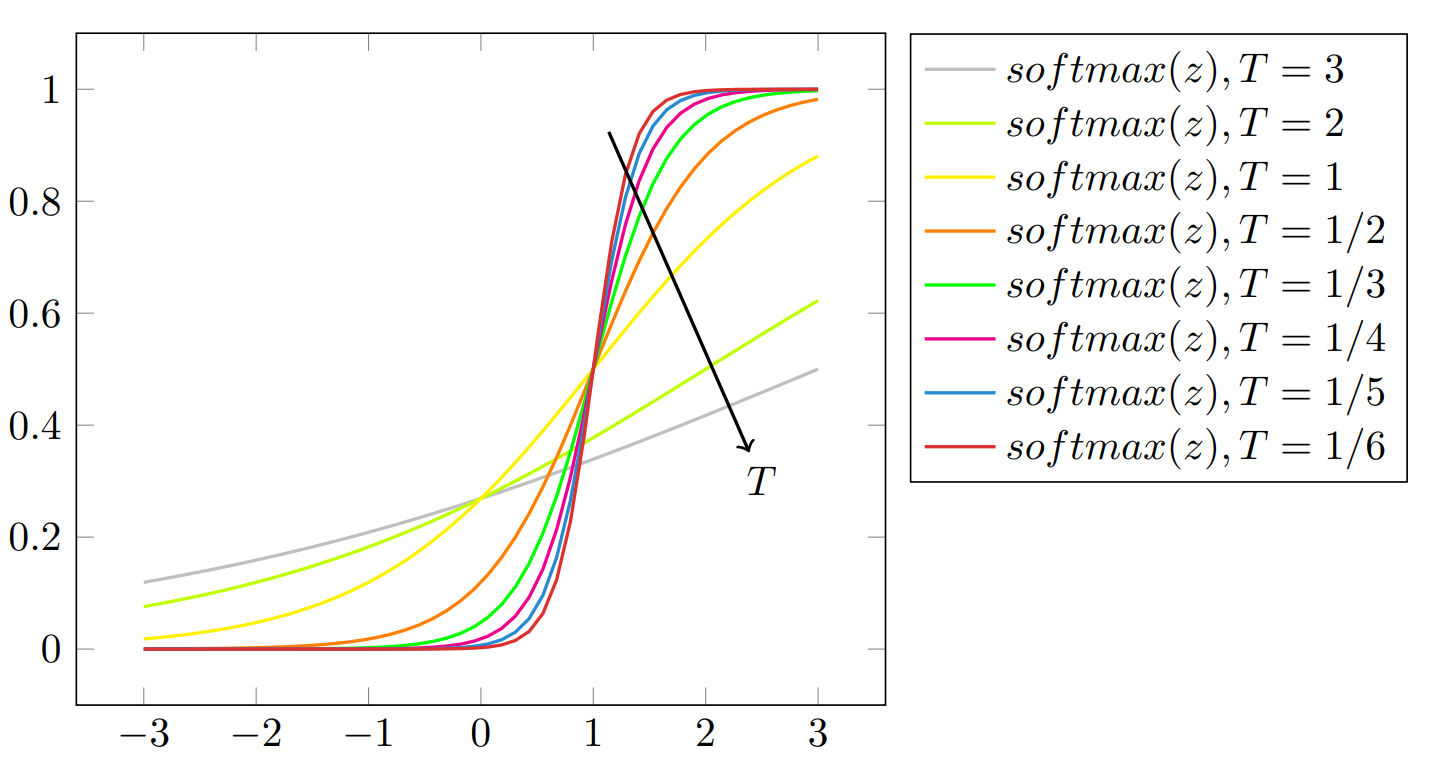
\includegraphics[width=\textwidth]{Figures/Softmaxbehaviour.png}
    \caption{The steepness of softmax function as temperature $T$ grows.}\label{fig:softmax}
\end{figure}

\section{Pooling}\label{sec:pooling}

In addition to convolutional , {\em pooling\/} operations
is an important building block in CNNs. Pooling operations reduce the spatial size of feature maps by using some aggregation, i.e) max or average, function to summarize a particular region.
The following properties affect the output size $o_j$ of a pooling layer
along axis $j$:

\begin{itemize}
    \item $i_j$: input size along axis $j$,
    \item $k_j$: pooling window size along axis $j$,
    \item $s_j$: stride (distance between two consecutive positions of the
        pooling window) along axis $j$.
\end{itemize}
\subsection{Average Pooling}
Average pooling is performed by sliding a window over the input feature map and performing and averaging the content of the window. Fig.~\ref{fig:numerical_average_pooling}
provides an example for average pooling.
\begin{figure}
    \centering
    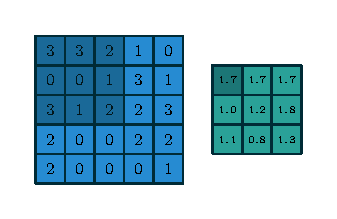
\includegraphics[width=0.32\textwidth]{pdf/numerical_average_pooling_00.pdf}
    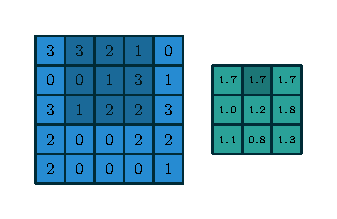
\includegraphics[width=0.32\textwidth]{pdf/numerical_average_pooling_01.pdf}
    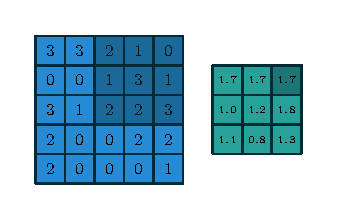
\includegraphics[width=0.32\textwidth]{pdf/numerical_average_pooling_02.pdf}
    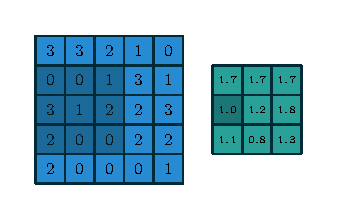
\includegraphics[width=0.32\textwidth]{pdf/numerical_average_pooling_03.pdf}
    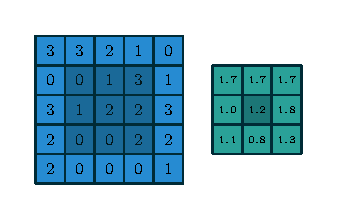
\includegraphics[width=0.32\textwidth]{pdf/numerical_average_pooling_04.pdf}
    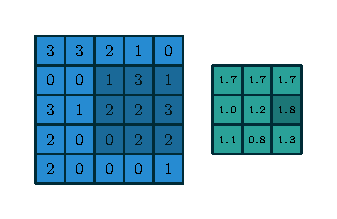
\includegraphics[width=0.32\textwidth]{pdf/numerical_average_pooling_05.pdf}
    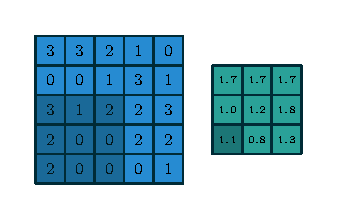
\includegraphics[width=0.32\textwidth]{pdf/numerical_average_pooling_06.pdf}
    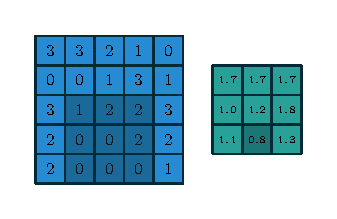
\includegraphics[width=0.32\textwidth]{pdf/numerical_average_pooling_07.pdf}
    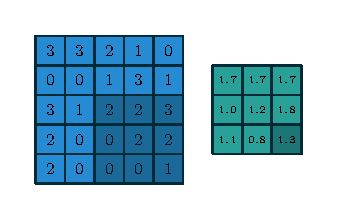
\includegraphics[width=0.32\textwidth]{pdf/numerical_average_pooling_08.pdf}
    \caption{\label{fig:numerical_average_pooling} Computing the output values
        of a $3 \times 3$ average pooling operation on a $5 \times 5$ input
        using $1 \times 1$ strides.}
\end{figure}



\subsection{Max pooling}
Max pooling is performed same way as the average pooling performed, but instead of performing the averaging as an aggregation function it performs max function. Fig.~\ref{fig:numerical_max_pooling} provides an example for average pooling.
\begin{figure}
    \centering
    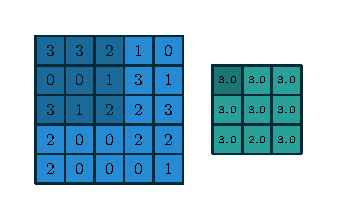
\includegraphics[width=0.32\textwidth]{pdf/numerical_max_pooling_00.pdf}
    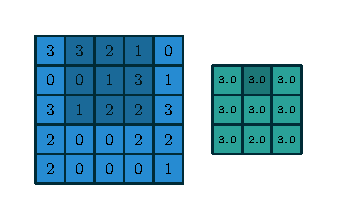
\includegraphics[width=0.32\textwidth]{pdf/numerical_max_pooling_01.pdf}
    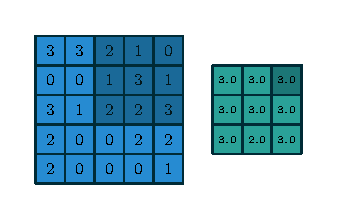
\includegraphics[width=0.32\textwidth]{pdf/numerical_max_pooling_02.pdf}
    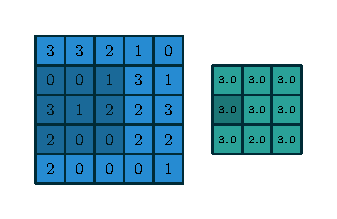
\includegraphics[width=0.32\textwidth]{pdf/numerical_max_pooling_03.pdf}
    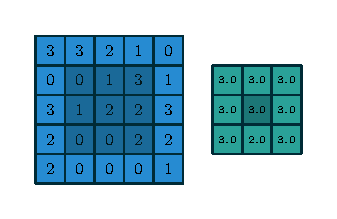
\includegraphics[width=0.32\textwidth]{pdf/numerical_max_pooling_04.pdf}
    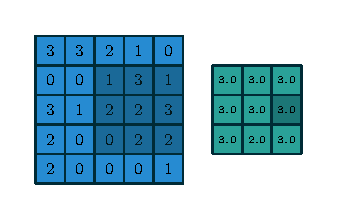
\includegraphics[width=0.32\textwidth]{pdf/numerical_max_pooling_05.pdf}
    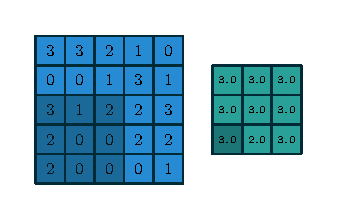
\includegraphics[width=0.32\textwidth]{pdf/numerical_max_pooling_06.pdf}
    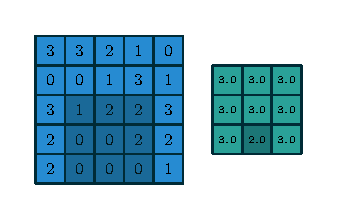
\includegraphics[width=0.32\textwidth]{pdf/numerical_max_pooling_07.pdf}
    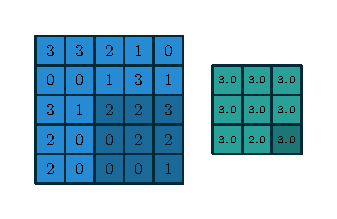
\includegraphics[width=0.32\textwidth]{pdf/numerical_max_pooling_08.pdf}
    \caption{\label{fig:numerical_max_pooling} Computing the output values of a
        $3 \times 3$ max pooling operation on a $5 \times 5$ input using $1
        \times 1$ strides.}
\end{figure}

CNN are used for feature extraction from images followed by fully connected layers for classification. As convolution operation is applied in a sliding window fashion it can accept input of varied size, resulting in a varied size output. As CNN is followed by fully connected layers which can accept input of fixed size. This makes CNN incapable of accepting varied size inputs. Thus images are first reshaped into some specific dimension before feeding into CNN. This creates another issue of image warping and reduced resolution. Spatial Pyramid pooling comes as a counter to this problem.

\section{Spatial Pyramid Pooling}

The convolutional layers process arbitrary variable length, and also they produce outputs of variable sizes. Classifiers like SVM, decision tree or fully-connected layers require fixed-length input feature vector. Such vectors can be generated by the Bag-of-Words (BoW) approach~\cite{sivic2003video} that pools the features together. Spatial pyramid pooling~\cite{grauman2005pyramid},~\cite{lazebnik2006beyond} improves BoW in where it can preserve the spatial information of the input by pooling local spatial bins. These spatial bins have sizes that are proportional to the input image, so the number of bins is fixed regardless of the input dimensions. While sliding window pooling of the previous deep networks~\cite{krizhevsky2012imagenet} the number of sliding windows depends on the input size. To adopt the deep network for images of arbitrary sizes, we replace the last pooling layer with a spatial pyramid pooling layer.
Fig.~\ref{originalSpp} illustrates our method. In each spatial bin, we pool the responses of each filter. The outputs of the spatial pyramid pooling are $kM$-dimensional vectors with the number of bins denoted as M (k is the number of filters in the last convolutional layer). The fixed-dimensional vectors are the input to the fully-connected layer. With spatial pyramid pooling, the input image can be of any sizes.
\begin{figure}
    \begin{center}
        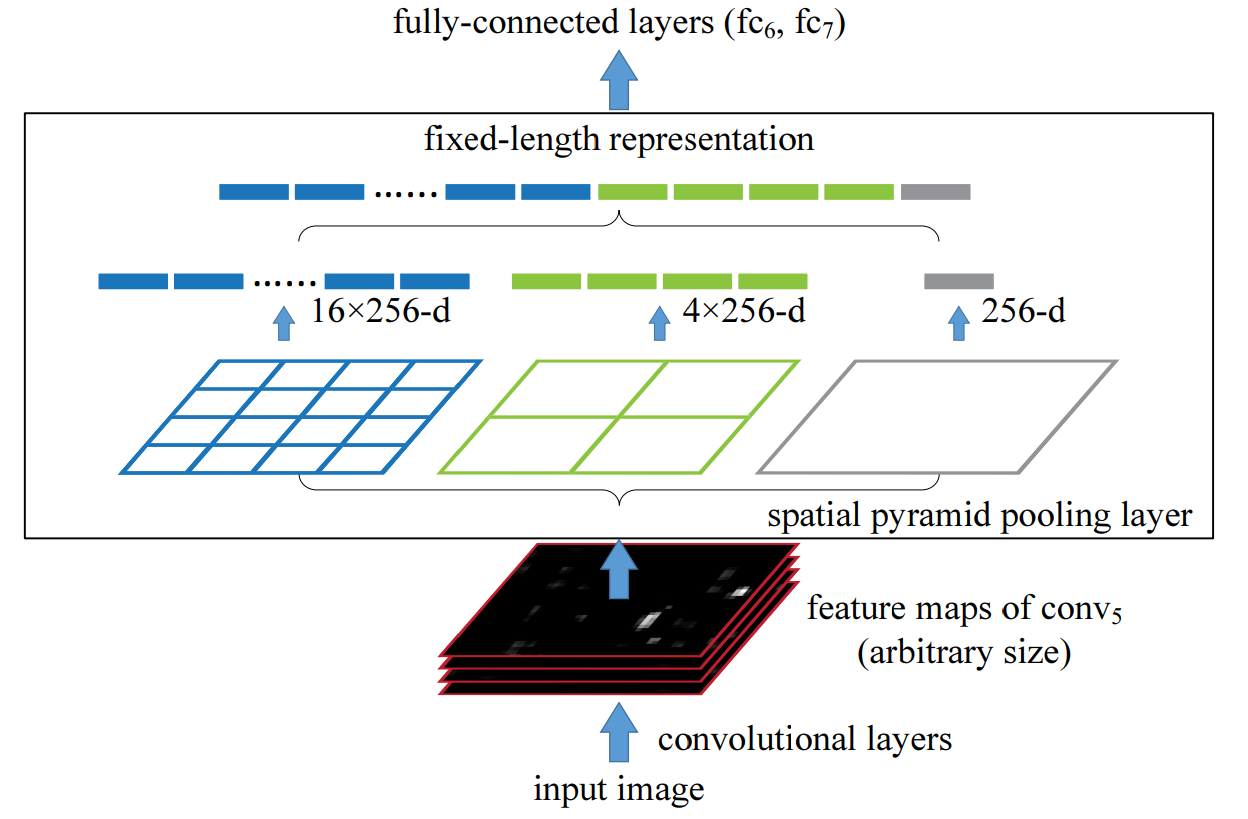
\includegraphics[width=\textwidth]{Figures/SPP.png}
        \caption{\label{originalSpp} spatial pyramid
        pooling layer. Input feature map is divided to pins for each pin an aggregation function is performed}
    \end{center}
\end{figure}

\section{Neural Network Attention}
In a vision system, an attention mechanism can be defined as a dynamic selection process that is realized by weighting features according to the importance of the input in an adaptive manner. Attention attempts to selectively concentrate on relevant information or features while ignoring other irrelevant ones.  Currently, attention based models have shown a great success in natural language processing \cite{vaswani2017attention} and computer vision tasks \cite{guo2022attention}. Attention modules guide the network to focus on the most relevant features only \cite{guo2022attention}. Attention has many categories such as channel attention and spatial attention. Stated as follows 
\subsection{Channel Attention}
Internal CNN feature maps have different channels in different usually each channel represents different objects~\cite{chen2017sca}. Channel attention recalibrates the weight of each channel, and can be viewed as an object selection process, thus determining what to pay attention to.~\cite{hu2018squeeze} is a pioneering channel attention mechanism which is formulated as follows
 \begin{equation}
    \begin{split}
        &Att(X) = \sigma(W_2ReLU(W_1GAP(X)))\\
        &Y = Att(X)X 
    \end{split}
\end{equation}
\noindent where $\sigma$ is sigmoid activation function, $GAP$ is global average pooling.
\begin{figure}
    \begin{center}
        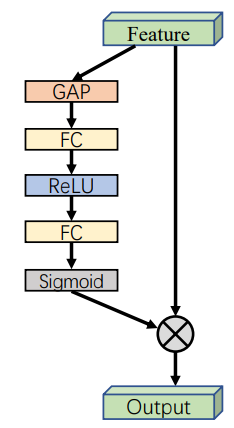
\includegraphics[width=.3\textwidth]{Figures/SE_attentBlock.png}
        \caption{\label{fig:SE_block} Channel attention block of SE network}
    \end{center}
\end{figure}
Fig.~\ref{fig:SE_block} illustrates the channel attention mechanism of~\cite{hu2018squeeze}
\subsection{Spatial Attention}
Spatial attention can be considered as an adaptive spatial region selection mechanism: where to pay attention.

In~\cite{woo2018cbam} generates a spatial attention map by utilizing the spatial relationship of features. Unlike channel attention, the spatial attention focuses on where is an informative part, which is complementary to the channel attention. They compute the spatial attention by first applying average-pooling and max-pooling operations over each channel and concatenate them to generate the  feature descriptor. After pooled-feature concatenation convolution layer is applied to generate a spatial attention map $\textbf{M}_{s}\left(F\right) \in \mathcal{R}^{H×W}$ which encodes the spatial importance.
We aggregate channel information of a feature map by using two pooling operations, generating two 2D maps:
$\mathbf{F}^{s}_{avg} \in \mathbb{R}^{1\times{H}\times{W}}$
and $\mathbf{F}^{s}_{max} \in \mathbb{R}^{1\times{H}\times{W}}$. Each denotes average-pooled features and max-pooled features across the channel. Those are then concatenated and convolved by a standard convolution layer, producing the 2D spatial attention map. In short, the spatial attention is computed as:
\begin{equation}\begin{split}
    &\textbf{M}_{s}\left(F\right) = \sigma\left(CONV_{7\times7}\left(\left[\text{AvgPool}\left(F\right);\text{MaxPool}\left(F\right)\right]\right)\right) \\
    &OR\\
    & \textbf{M}_{s}\left(F\right) = \sigma\left(CONV_{7\times7}\left(\left[\mathbf{F}^{s}_{avg};\mathbf{F}^{s}_{max} \right]\right)\right) 
\end{split}\end{equation}
where $\sigma$ denotes the sigmoid function,  $CONV_{7\times7}$ represents a convolution operation with the filter size of $7\times7$, and $[\cdot]$ is a concatenation operator.
\begin{figure}
    \begin{center}
        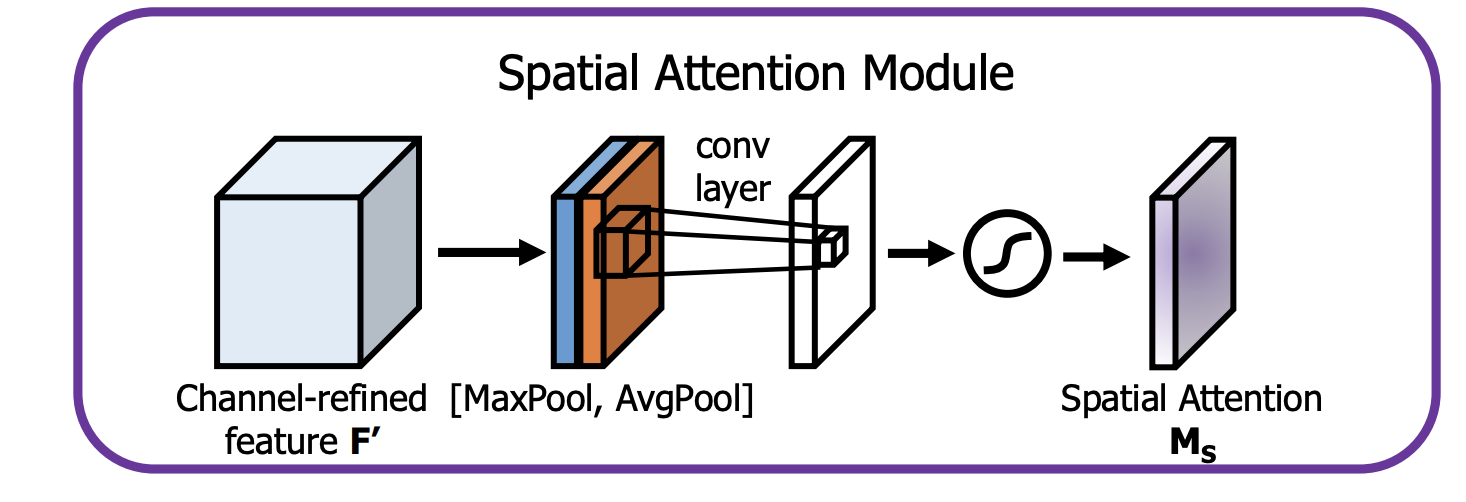
\includegraphics[width=\textwidth]{Figures/SpatialAttentionExample.png}
        \caption{\label{fig:spattex} Spatial attention mechanism }
    \end{center}
\end{figure}

\section{Normalization}
Normalization is crucial for training a deep network. Normalization allows the use of larger learning rate and results in smoother loss landscape of the objective function. Different types are summarized as follows:
\subsection{Batch Normalization}
As proposed in~\cite{ioffe2015batch} batch normalization is reduces {\em  Internal Covariate Shift} (ICS). ICS is defined as the change in the distribution of network activations due to the change in network parameters during training. Batch Normalization (BN) mitigate the ICS by normalizing the internal feature maps, minibatch, to have zero mean and unit variance. BN also allows the CNN to undo the normalization by scaling and shifting the normalized features using $\gamma$, $\beta$. 

BN is applied to each layer for a minibatch $\mathcal{B}$ as follows:
\begin{equation}
\begin{split}
    & \mu_{\mathcal{B}} = \frac{1}{m}\sum^{m}_{i=1}x_{i}\\
    &  \sigma^{2}_{\mathcal{B}} = \frac{1}{m}\sum^{m}_{i=1}\left(x_{i}-\mu_{\mathcal{B}}\right)^{2}\\
    &  \hat{x}_{i} = \frac{x_{i} - \mu_{\mathcal{B}}}{\sqrt{\sigma^{2}_{\mathcal{B}}+\epsilon}} \\
    &  y_{i} = \gamma\hat{x}_{i} + \beta = \text{BN}_{\gamma, \beta}\left(x_{i}\right) \\
\end{split}
\end{equation}
BN has many benefits which is summarized as follows:
\begin{itemize}
    \item \textbf{Accelerate network training.} BN allows larger learning rate.
    \item \textbf{Regularization effect.} BN has regularization effect due to batch construction is done stochastically.
    \item \textbf{Mitigate the effect of saturating activation function.} Normalization performed by BN relocate the layer activation to linear regime of saturating activation function such as sigmoid.
\end{itemize}

\subsection{Layer Normalization}

Unlike batch normalization, Layer Normalization~\cite{ba2016layer} directly estimates the normalization statistics from the summed inputs to the neurons within a hidden layer so the normalization does not introduce any new dependencies between training samples.

We compute the layer normalization statistics over all the hidden units in the same layer as follows:

\begin{equation}
\begin{split}
    & \mu^{l} = \frac{1}{H}\sum^{H}_{i=1}a_{i}^{l}\\
    &  \sigma^{l} = \sqrt{\frac{1}{H}\sum^{H}_{i=1}\left(a_{i}^{l}-\mu^{l}\right)^{2}} \\
\end{split}
\end{equation}
where $H$ denotes the number of hidden units in a layer. Under layer normalization, all the hidden units in a layer share the same normalization terms $\mu$ and $\sigma$, but different training samples have different normalization terms. Unlike batch normalization, layer normalization does not impose any constraint on the size of the mini-batch and it can be used in the pure online regime with batch size of 1 sample.

\section{Augmentation}
Data augmentation~\cite{balestriero2022effects} is a technique that is  used for enlarging the training set, based on different modifications, using label preserving transformation. Data augmentation not only helps to grow the dataset but it also increases the diversity of the dataset and introduce  robustness to these transformations. When training machine learning models, data augmentation acts as a regularizer and helps to avoid overfitting.

Data augmentation techniques have been found useful in domains like NLP and computer vision. In computer vision, transformations like cropping, flipping, and rotation are used. Fig. \ref{fig:DADeg} represents pre-class performance to the degree of augmentation.
\begin{figure}
    \begin{center}
        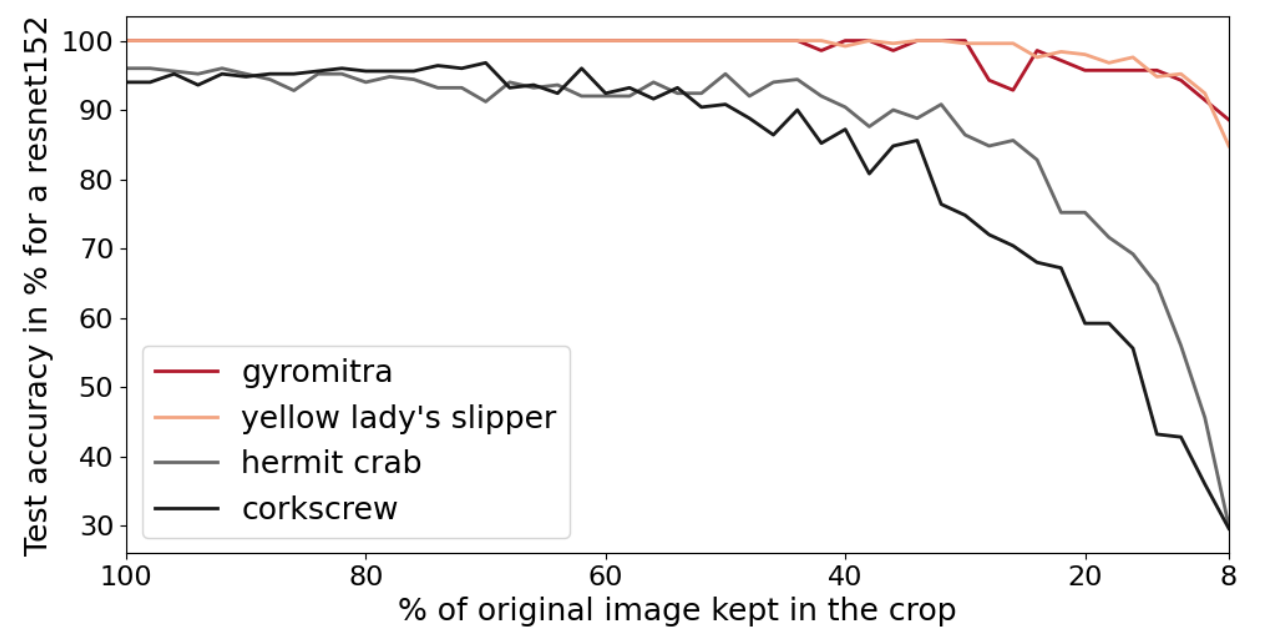
\includegraphics[width=\textwidth]{Figures/labelpreserveAug.png}
        \caption{\label{fig:DADeg}Data augmentation using crop augmentation with different preserving degrees and the corresponding accuracy of recognizing certain classes using ResNet}
    \end{center}
\end{figure}


\section{Dropout}


\begin{figure}
    \begin{center}
        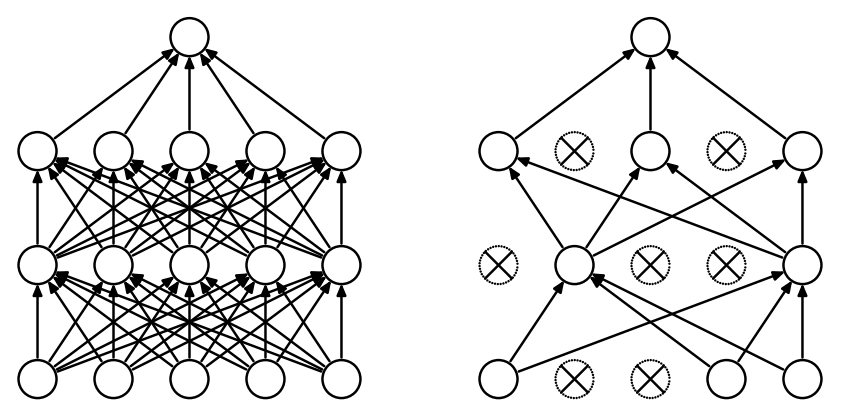
\includegraphics[width=\textwidth]{Figures/oriDropout.png}
        \caption{\label{fig:Dropout} Dropout Neural network Model. \textbf{Left}: A standard network with two hidden layers. \textbf{Right}: An example of a thinned net produced by applying dropout to the network on the left. Crossed units have been dropped.}
    \end{center}
\end{figure}
Dropout~\cite{srivastava2014dropout} is a regularization technique for neural networks that drops a unit (along with connections) at training time with a specified probability $p$ (a common value is $p=0.5$). At test time, all units are present, but with weights scaled by $p$ (i.e. $w$ becomes $pw$).
Dropout has the following benefits. 
\begin{itemize}
    \item \textbf{Reduces co-adaptation between the neurons.} Complex co-adaptation between neuron occurs when the neurons of the one layer depend on the neurons on next layers to correct their errors. Dropout fixes this issue by making neuron existance stochastic.
    \item \textbf{Implicit ensemble.} Dropout  approximately combining exponential number different thinned neural network architectures efficiently
\end{itemize}
Fig.~\ref{fig:Dropout} illustrates the operation of the Dropout.

\section{Multiscale Recognition}
CNN,  like many computer vision models, is a scale-variant \cite{van2017learning} model such that it cannot recognize objects at various scales unless it explicitly trained to recognize such objects. Many approaches have been developed to overcome this problem. The first approach is referred to as \textit{shared-net}. Shared-net approach creates a scale-pyramid of the input image  to train a single shared network using  multiple scales. This shared network produces a feature vector for each scale which in turn is fused with an aggregation function to produce the final prediction \cite{farabet2012learning}\cite{lin2016efficient}\cite{felzenszwalb2009object}\cite{ciregan2012multi}. Shared-network needs to evaluate each scale independently which is a time-consuming.

The second approach is to reuse low level features produced by the intermediate CNN layers using a skip connection \cite{chen2014semantic}\cite{hariharan2015hypercolumns}. These features are considered multi-scale due to the different receptive field of the corresponding layers. The training of these networks is performed through two phases. Backbone network is trained in the first phase.  Then, it is fine-tuned during multi-scale feature extraction \cite{long2015fully}\cite{lin2017feature}. The drawback of this approach is the separation between the classifier training and the feature extraction.\\
\begin{center}
    \begin{figure}
    \centerline{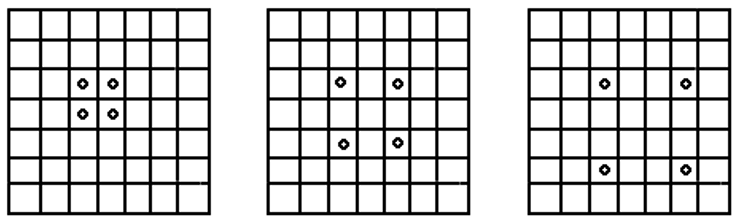
\includegraphics[width=\textwidth]{Figures/AtrousConv.PNG}}
    \caption{A grid represents a feature map and the circle inside the cell represents the corresponding value of $2\times 2$ convolutional kernel. \textbf{left}: A $2\times 2$ convolutional kernel with an atrous rate $r=1$. \textbf{middle}: A $2\times 2$ convolutional kernel with an atrous rate $r=2$. \textbf{right}: A $2\times 2$ convolutional kernel with an atrous rate $r=3$.}
    \label{AtrousConv}
    \end{figure}
    \end{center}
The third and the  recent approach is to deploy atrous convolution \cite{holschneider1990real} in CNN context \cite{chen2017deeplab}\cite{giusti2013fast}. Atrous convolution is defined as follows: \[y[i]=\sum_{k}^{K} x[i+r\times k] w[k]\] where $x$ is the input signal, $w$ is the convolutional filter with size of $K$, $y$ is the resultant signal, and $r$ is the atrous rate. Atrous convolution can be seen as a convolution  operation between the input signal and the upsampled version of the filter. This upsampling is performed by introducing $r-1$ zeros between the kernel values. Also, Atrous convolution can be seen as a  convolution between the downsampled version of the input signal and the kernel. Atrous convolution allows the change in the receptive field and controls the input signal resolution without increasing the parameter number \cite{chen2017rethinking} (\textit{i.e,} a $3\times 3$ convolutional kernel and a dilation rate of $r=2$ has the same receptive field of $5\times 5$ convolutional kernel and dilation rate of $r=1$). Atrous convolution can be used to build the resultant scale-space through  performing Atrous convolution with multiple Atrous rates, $r$, which is known as Atrous Spatial pyramid Pooling (ASPP) \cite{chen2017deeplab}. ASPP has a regularization effect as it ensures that the convolutional kernels will learn  useful features   across the scale space of the input. Fig. \ref{AtrousConv} shows an example of  Atrous convolution with different rates. 


% \section{Initialization}

% \section{Optimization}

\section{Summary}
CNN is currently a state-of-the-art of many computer vision problems. CNN 
In this chapter a required background to understand the proposed work is presented. Basic building blocks of CNN is illustrated and recent technique required to efficiently train the CNN is illustrated.
